\section{Результаты}

\subsection{Качество аудио}

Одна из самых больших проблем с разработкой систем для генерации речи это отсутствие быстро (программно) вычислимой метрики, которая хорошо коррелирует с качеством произношения. Зачастую, в процессе разработки, качество приходиться мерить "на слух", замедляя таким образом исследования и ухудшая реальную требуемую корреляцию с человекоподобной речью. Для того, чтобы оценить качество TalkNet, следуя другим работам~\cite{fastspeech, tacotron2}, было решено провести случайный слепые тесты с дискретным оцениванием и усреднить результаты для того, чтобы получить примерное представление о работоспособности получившейся модели.

Для оценки качества был проведен эксперимент MOS (mean opinion score) для сгенерированной речи с использованием Amazon Mechanical Turk~\cite{mturk}. Сравнивались четыре набора подходов к генерации для тестовой части датасета LJSpeech: 1) Истинные аудио с речью; 2) Истинные мэл-спектрограммы, преобразованная в речь с помощью WaveGlow; 3) Tacotron 2 + WaveGlow и 4) TalkNet + WaveGlow. Были использованы реализации NVIDIA для Tacotron 2 и WaveGlow. Тестировались $100$ аудио примеров, где каждый пример был оценен не менее $10$ раз $10$ различными людьми. Также, были использованы дополнительные фильтры для отсева людей без высшего образования или людей не знающих английский язык для повышения стабильности оценивания. Оценивающим предлагалось проверить работоспособность гарнитуры, несколько раз прослушать отрывок и выбрать наиболее подходящую оценку на вопрос "насколько представленный отрывок похож на человеческую речь?". Баллы варьировались от $1.0$ до $5.0$ с шагом $0.5$ (всего -- 9 ступеней). Как можно заметить, качество речи TalkNet сравнимо к Tacotron 2 (Таблицы~\ref{tab:mos}).

\begin{table}[!ht]
\centering
\scalebox{1.5}{
\begin{tabular}{l c} 
\toprule
\textbf{Model} &
\textbf{MOS} \\
\midrule
Ground truth speech & $4.31 \pm 0.05$ \\
Ground truth mel + WaveGlow & $4.04 \pm 0.05$ \\
Tacotron 2 + WaveGlow & $3.85 \pm 0.06$ \\
\midrule
TalkNet + WaveGlow & $3.74 \pm 0.07$ \\
\bottomrule
\end{tabular}
}
\caption{Усредненные оценки MOS (mean opinion score) с $95\%$ доверительным интервалом}
\label{tab:mos}
\end{table}

Одна из дополнительных характеристик генерации, помимо качества звучания, это способность модели не пропускать слова и правильно произносить имеющиеся даже при сложных входных строках. Такая характеристика называется устойчивостью (robustness). Следуя FastSpeech~\cite{fastspeech}, были проведены эксперименты для сравнения устойчивости различных моделей на $50$ особенно сложных для генерации входных предложениях~\ref{fig:hard-examples}, считая вручную количество пропущенных или повторенных слов. Данные предложения представляют особенную сложность, из-за отсутствия правдоподобного контекста, поэтому генеративной модели приходится выводить корректное произношение почти побуквенно. В результаты экспериментов было обнаружено, что подобно FastSpeech, TalkNet устраняет ошибки связанные с пропущенными или повторяющимися словами. Таким образом, неавторегрессионый подход очень устойчив и не имеет ошибок с отсутствующими или повторяющимися словам, что делает его более выгодным по сравнению с авторегрессионными моделями TTS, такими как Tacotron 2 или Transformer TTS.

\begin{figure}[!ht]
\centering
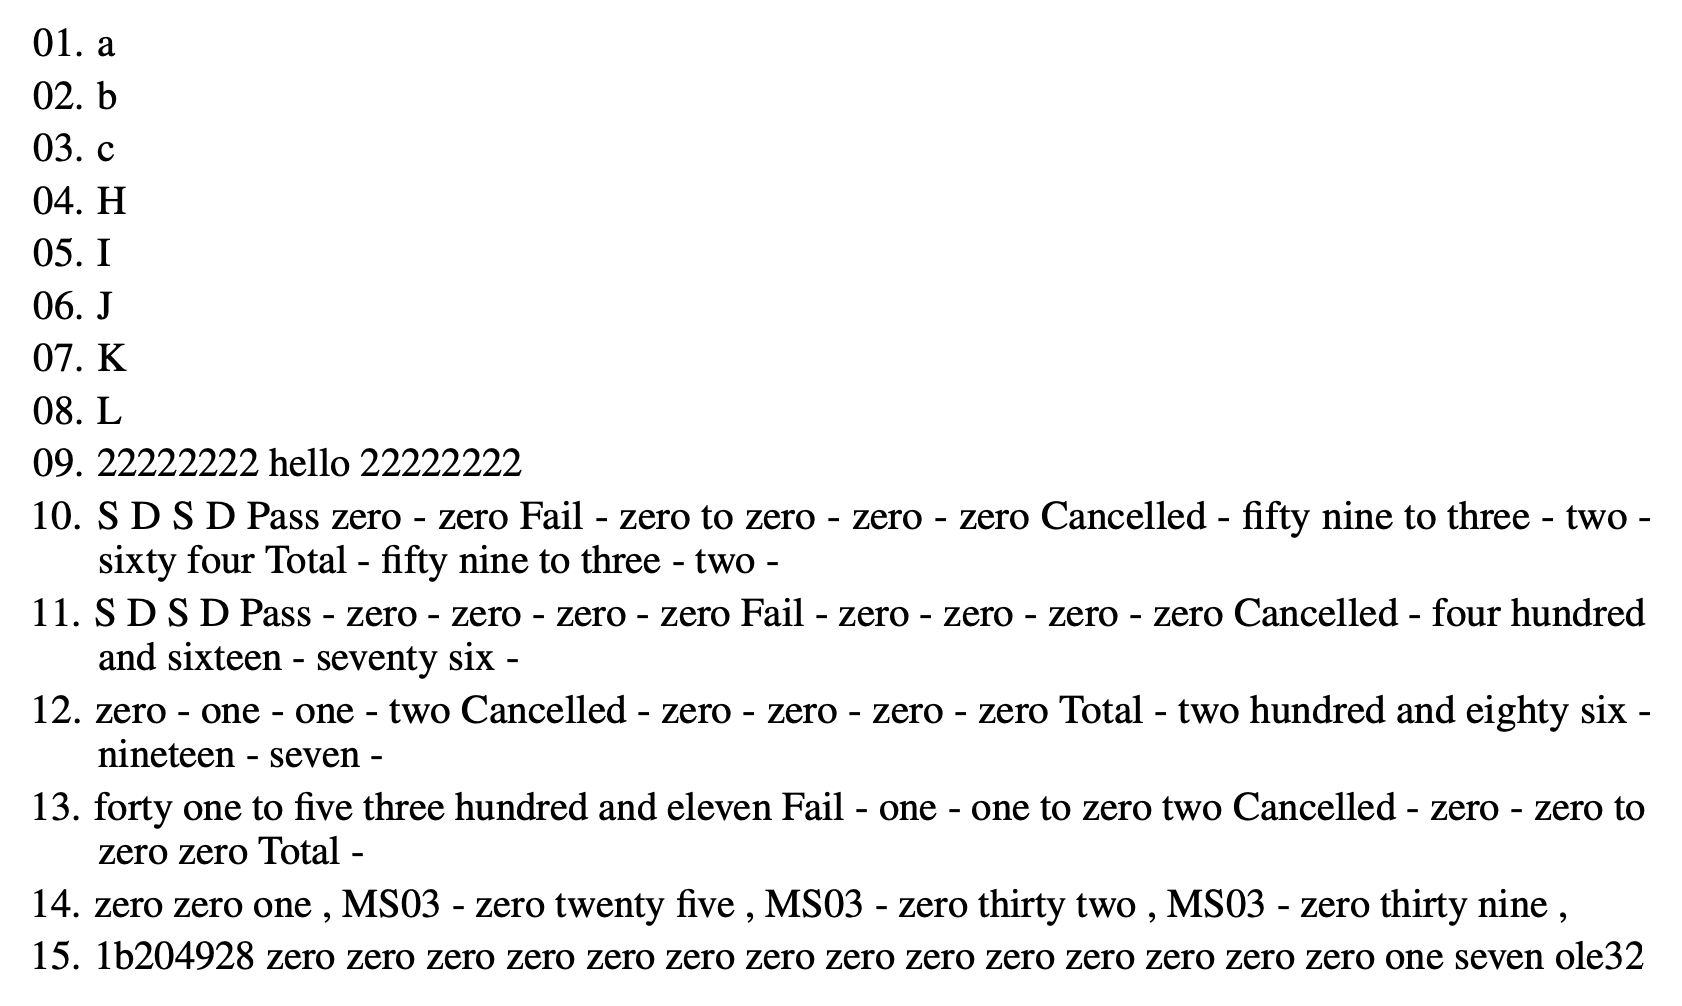
\includegraphics[width=1.0\textwidth]{images/snippets/hard-examples.png}
\caption{Первые 15 из 50 сложных примеров для проверки генерации TTS систем}
\label{fig:hard-examples}
\end{figure}

\subsection{Скорость генерации}

Процесс вывода (inference) TalkNet описан на Рисунке~\ref{fig:arch}. Сначала, вставляются пустые символы в входной текст между каждыми двумя соседними. Полученная последовательность пропускается через предиктор длительностей графем. Входные данные предиктора длительностей затем корректируются для символов с длительностью $0$. Так избегаются неправильные предсказания длительностей для редких символов (знаков препинания), что позволяет оставить их после операции расширения. Исправленная последовательность символов расширяется при повторении каждого символа в соответствии с предсказанной длительностью. Вторая часть модели генерирует мэл-спектрограмму из развернутой последовательности графем, равной ей по длине.

Такой процесс имеет несколько узких мест с точки зрения скорости:
\begin{itemize}
    \item Матричные операции, необходимые для вывода предиктора длительностей.
    \item Матричные операции, необходимые для вывода генератора мэл-спектрограмм.
    \item Передача и трансформация данных между частями.
\end{itemize}

Очевидно, что все части вывода по времени зависят от длины текста и соответствующего мэла. Поэтому, для правильного сравнивания TTS систем для генерации речи замерялась задержка (latency), необходимая всем частям системы суммарно на получение мэл-спектрограммы. Получившиеся задержки усреднялись ее по множеству примеров с различной длиной. Заметим также, что этап вокодинга не включен во время задержки, но все еще необходим для построения полной системы для генерации речи. Обычно, вокодинг занимает в десятки раз больше времени и весов, поэтому все еще является узких местом всей системы.

Были сравнены задержки вывода TalkNet с Tacotron 2 и FastSpeech. Использовались реализации FastSpeech от NVIDIA, так как исходная код был недоступен на момент оценки. Чтобы измерить задержку, были сгенерированны мэл-спектрограммы с размером батча, равным 1 и проводим усреднение по 2048 образцам из тестового набора данных LJSpeech. Средняя длина мэл-спектрограммы при таком подходе составляет $520$. Сравнивались задержки используя один и то же аппаратное оборудование (hardware) -- один графический процессор V100. Как можно видеть, скорость вывода TalkNet значительно быстрее, чем Tacotron 2 и FastSpeech (Таблица~\ref{tab:lats}). Если же проводить вывод по 4 или 8 примеров за раз, то скорость повышается линейно, достигая $1300$ RTF.

\begin{table}[!ht]
\centering
\scalebox{1.2}{
\begin{tabular}{l l l r} 
\toprule
\textbf{Model} & 
\textbf{\thead{\# Batch\\size}} &
\textbf{\thead{Inference\\Latency, s}} &
\textbf{RTF} \\
\midrule
Transformer TTS~\cite{transformer-tts} & 1 & $6.735 \pm 3.969$ & $1.48 \pm 0.87$ \\
Tacotron 2~\cite{tacotron2} & 1 & $0.817 \pm 1\cdot 10^{-2} $ & $7.56 \pm 0.01$ \\
FastSpeech~\cite{fastspeech} & 1 & $0.029 \pm 2 \cdot {10}^{-4}$  & $221.01 \pm 1.75$ \\
\midrule
TalkNet & 1 & $0.019 \pm 1 \cdot {10}^{-5}$ & $328.65 \pm 4.76$ \\
TalkNet & 4 & $0.023 \pm 5 \cdot {10}^{-5}$ & $1048.80 \pm 21.75$ \\
TalkNet & 8 & $0.037 \pm 4 \cdot {10}^{-4}$ & $1340.09 \pm 8.90$ \\
\bottomrule
\end{tabular}
}
\caption{Задержка вывода TalkNet для генерации мэл-спектрограммы (без вокодера). Задержка была измерена с размером батча $1$ с использованием графического процессора V100 и усреднена по 2048 примерам из набора данных LJSpeech. Приведены усредненное время задержки и фактор реального времени (RTF) с доверительным интервалом $95\%$. Фактор реального времени показывает сколько секунд речи можно сгенерировать за одну секунду вычислений.}
\label{tab:lats}
\end{table}

Поскольку TalkNet не использует операции с механизмами внимания (attention), задержка вывода практически не зависит от длины входного сигнала~\ref{fig:len-lat}. Операции c attention обычно реализуются с перемножением матриц, вытянутых по длине вывода. Поэтому, такая операция занимает порядка $O(T^2)$ операция, что приводит к линейному росту времени при парралелизации на графических ускорителях ГПУ.

\begin{figure}[!ht]
\centering
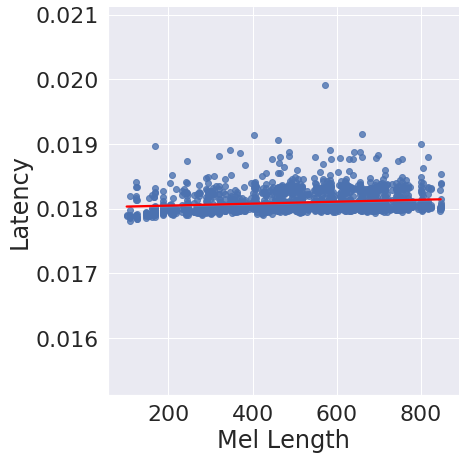
\includegraphics[width=0.8\textwidth]{images/len-lat.png}
\caption{Влияние неавторегрессионной архитектуры и отсутствия механизмов внимания}
\label{fig:len-lat}
\end{figure}

Стоит также отметить, что текущим самым узким местом с точки зрения скорости вывода TalkNet является непосредственные вычисления операций нейронной сети (конволюции, нелинейности, батч нормализация, дропаут). Однако, текущие реализации CUDA кернелов (специальных функций для вычислений операций на графических ускорителях) для depthwise separable конволюций, из которых почти полностью состоит TalkNet, написаны не самым оптимальным образом. Полагается, что написание оптимальных функций для 1d time и 1x1 pointwise сверток с использованием идей fusing'а (когда две последовательные операции сокращаются в одну) может значительно ускорить работу предложенной модели.